% Nama Kelompok : Kelompok 3
% Kelas : D4 TI 1A
% 1. Kadek Diva Krishna Murti (1174006)
% 2. Niko
% 3. Rizal Rony Sitorus
% 4. Jeremia Wahyudi Sianturi (1174029)
% 5. Sri Rahayu (1174015)

\section{Pengertian Bit Parity}
Bit Parity merupakan bit tambahan yang disisipkan pada urutan bit-bit data yang ditransmisikan.
Tujuan pemberian bit parity ini adalah untuk memastikan bahwa bit - bit yang ditransmisikan tidak mengalami perubahan nilai setelah sampai di penerima.
Perubahan nilai dapat terjadi karena pengaruh noise atau sinyal liar.
Perubahan nilai : 0 $\,\to\,$ 1 atau 1 $\,\to\,$ 0
\newline Contoh :

\begin{table}[h!]
\centering
\begin{tabular}{ c c c }
0110100 & $\,\to\,$ &  0100100\\
\hline
Tx &  & Rx \\
\end{tabular}
\end{table}

\begin{figure}[ht]
\centerline{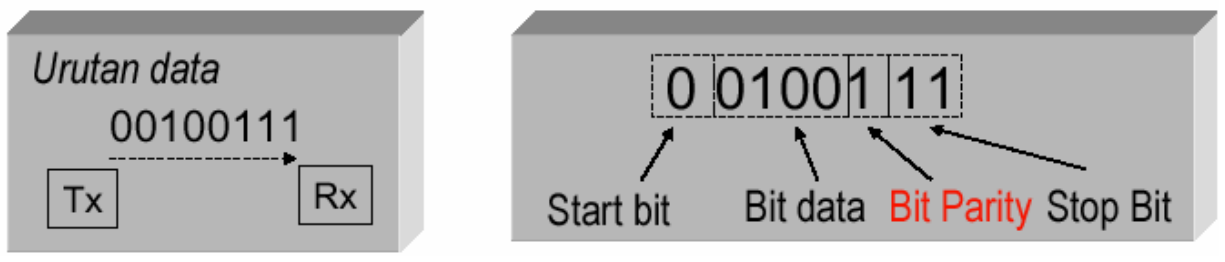
\includegraphics[width=1\textwidth]{figures/perubahan_nilai_bit_parity.png}}
\caption{Contoh perubahan nilai pada bit parity.}
\label{perubahan_nilai_bit_parity}
\end{figure}

Proses perubahan nilainya bisa dilihat pada gambar \ref{perubahan_nilai_bit_parity}

\section{Cara Kerja Bit Parity}
\subsection{Konsep Umum}
Pihak pengirim akan menambahkan 1 bit tambahan (Bit Parity) pada data, untuk menggabarkan karakteristik dari data tersebut. Nilai dari bit parity (1 atau 0) tidak diperbolehkan secara sembarang. Dalam proses pentransmisiannya data tadi dikirim bersamaan (data dan bit parity-nya). Pada terminal penerimaan data kita dibaca dan di dekodisasi dengan cara yang sama seperti saat menentukan nilai bit parity disisi pengirim. Lalu hasil dekodisasi tadi dibandingkan dengan bit parity yang dibawakan oleh pengirim.
Apabila hasil pembacaan (dekodisasi) data terkirim sama dengan bit Paritynya maka data tersebut dapat dianggap benar. Dan apabila diperoleh perbedaan nilai antara hasil dekodisasi dengan bit Paritynya maka data dapat di klasifikasi sebagai data yang error. Terminal penerima akan mengirim request pada terminal pengirim untuk mengirim ulang data yang error.
 
\subsection{Menentukan Nilai Bit Parity}
Penentuan nilai bit Parity (1 atau 0) dilakukan dengan meng-XOR kan semua bit yang ada pada data sepasang-sepasang, hasil akhir dari peng-XOR an seluruh bit ini yang akan dijadikan acuan untuk menentukan nilai dari bit Parity yang akan ditambahkan. Jadi belum tentu hasil XOR langsung dijadikan sebagai nilai dari bit Parity.


%%%%%%%%%%%%%%%%%%%%%%%%%%%%%%%%%% KADEK DIVA KRISHNA MURTI %%%%%%%%%%%%%%%%%%%%%%%%%%%%%%%%%%%%%

\section{Kelebihan dan Kekurangan Bit Parity}
\subsection{Kelebihan Bit Parity}
-   Lebih cepat karena berbasis 2 (biner)
-   Mudah dalam pengecekan
-   Sederhana dalam analisis dan penggunaan pada sistem
-   Mudah direalisasikan dalam bentuk rangkaian atau hardware

\subsection{Kekurangan Bit Parity}
-   Kurang handal dalam mengatasi deteksi dan perbaikan error
-   Kemungkinan kesalan yang terjadi besar, yaitu 50%
-   Belum dapat mengakomodir file dengan ukuran besar
-   Tidak dapat mendeteksi kesalahan dalam jumlah genap



\section{Pembagian Jenis Bit Parity}
\subsection{Parity Ganjil}
Bit Paritas di set menjadi 1 apabila jumlah angka 1 dalam kesatuan bit tersebut (tidak termasuk bit paritas) adalah genap, sehingga menjadikan jumlah bit dalam kesatuan tersebut (termasuk bit paritas) menjadi ganjil.
 
\subsection{Parity Genap}
Bit paritas di set menjadi 1 apabila jumlah angka 1 dalam kesatuan tersebut (tifak termasuk bit paritas) adalah ganjil, sehingga menjadikan jumlah bit dalam kesatuan tersebut (termasuk bit paritas) menjadi genap.

%%%%%%%%%%%%%%%%%%%%%%%%%%%%%%%% NICO EKKLESIA SEMBIRING %%%%%%%%%%%%%%%%%%%%%%%%%%%%%%%%%%%%%%%

\section{Sejarah Bit Parity}
Sebuah "paritas track" hadir pada penyimpanan data pita magnetik pertama pada tahun 1951. Paritas dalam bentuk ini, diterapkan di beberapa sinyal paralel, dikenal sebagai cek redundansi transversal. Ini dapat dikombinasikan dengan paritas yang dikomputasi melalui beberapa bit yang dikirim pada sinyal tunggal, pemeriksaan redundansi longitudinal. Dalam bus paralel, ada satu bit cek redundansi longitudinal per sinyal paralel.
Paritas juga digunakan pada setidaknya beberapa sistem pemasukan pita kertas (tape berlubang) (yang mendahului sistem pita magnetik). Pada sistem yang dijual oleh perusahaan Inggris ICL (sebelumnya ICT), pita kertas berukuran 1 inci (25 mm) memiliki 8 posisi lubang yang melintang di atasnya, dengan posisi ke 8 untuk paritas. 7 posisi digunakan untuk data, misalnya, 7-bit ASCII. Posisi 8 memiliki lubang yang dilubangi tergantung pada jumlah lubang data yang dilubangi.